\section{Saga Execution Component}

In \ref{sec_Services} wurde festgelegt, dass der OrderService die Rolle des Koordinators übernimmt. Das bedeutet, dass der OrderService die Saga Execution Component enthält. Als solche hat der OrderService die Verantwortung, die an der LLT teilhabenden Services aufzurufen und auf die Ergebnisse zu reagieren. In diesem Abschnitt werden die dafür notwendigen Implementierungsdetails dargestellt.

\subsection{Rahmenbedingung für die Versuchsdurchführung}
Die SEC übernimmt die Aufgabe, einen DEA auszuführen. Im Rahmen des Versuchs sollen mehrere DEAs konstruiert und durch die selbe SEC ausgeführt werden. Die SEC muss also flexibel genug implementiert werden, damit eine Parametrisierung der Ausführung mit einem DEA als Argument möglich ist. 

\subsection{Ausführung eines DEAs}
Zunächste soll der Ablauf eines Durchlaufs eines DEAs innerhalb der SEC dargestellt werden. Es soll nun davon ausgegangen werden, dass ein DEA definiert wurde. 

\begin{enumerate}
	\item Nach Eingang einer Bestellung wird der Initialzustand gewählt, um die Ausführung des DEAs zu starten.
	\item Jeder Zustand korrespondiert mit einer auszuführenden Aktion. Diese Aktion wird ausgeführt. 
	\item Eine Aktion resultiert in einem Ergebnis. Dieses Ergebnis stellt ein Element aus der Menge des Eingabealphabets dar. Dieses Element wird zusammen mit dem Zustand in der Datenbank gespeichert. 
	\item Die Ausführung des Zustands wird beendet.
	\item Die SEC bestimmt den nächsten Zustand. Und führt die korrespondierende Aktion aus.
	\item Die Aktion resultiert in einem Ergebnis. Das Ergebnis wird in der Datenbank gespeichert. 
	\item Die Ausführung des Zustands wird beendet. 
	\item Die SEC wiederholt diesen Prozess solange bis ein Endzustand erreicht wird. 
\end{enumerate}

\subsection{Modellierung eines DEAs}
Die Modellierung eines DEAs ist in \cref{lst:dea-model-csharp} abgebildet. 

\begin{lstlisting}[breaklines=true, tabsize=2, showstringspaces=false, frame=single, numbers=left, basicstyle=\small, label = {lst:dea-model-csharp}, caption={Modellierung eines DEA in C\#}, captionpos=b] 
public class SimpleStateMachine
{
	public List<string> States;
	public string InitialState;
	public List<string> EndStates;
	public List<string> Sigma;
	public List<Tuple<Tuple<string, string>, string>> Relations;
	
	
	public SimpleStateMachine(List<string> states,
		string initialState,
		List<string> endStates,
		List<string> sigma,
		List<Tuple<Tuple<string, string>, string>> relations)
	{
		States = states;
		InitialState = initialState;
		EndStates = endStates;
		Sigma = sigma;
		Relations = relations;
	}
}
\end{lstlisting}

\paragraph*{Relations} \mbox{}\\
Das Feld \textit{Relations} stellt Liste von möglichen Zustandsübergängen dar. Die SEC kann aus einem Zustand und einem Element aus Sigma den entsprechenden Zustandsübergang berechnen. Damit diese Berechnung deterministisch ist, darf für einen gegebenen Zustand und einen gegebenes Element aus Sigma nur ein Element existieren. 

\subsection{Konstruktion eines DEAs}
Nun soll ein solcher DEA initialisiert werden. Dazu wird der Konstruktor dieser Klasse aufgerufen. Es soll folgender Automat konstruiert werden:

\begin{figure}[ht!]
	\centering
	\begin{tikzpicture}[->,>=stealth',shorten >=1pt,auto,node distance=2.5cm, semithick]
		\node [state, initial] 		(qt1) 					{$q_{t1}$};
		\node [state] 				(qt2) [right of=qt1] 	{$q_{t2}$};
		\node [state] 				(qt3) [right of=qt2] 	{$q_{t3}$};
		
		\node [state] 				(qc1) [below of=qt2] 	{$q_{c1}$};
		\node [state] 				(qc2) [right of=qc1] 	{$q_{c2}$};
		
		\node [state, accepting] 	(qf1) [right of=qt3] 	{$q_{f1}$};
		\node [state, accepting] 	(qf2) [left of=qc1] 	{$q_{f2}$};
		\node [state, accepting] 	(qf3) [below of=qc2] 	{$q_{f3}$};
		
		\path (qt1) 	edge					node 		{$t1_{200}$}		(qt2)
						edge					node		{$t1_{400}$}		(qf2)
		(qt2)			edge					node		{$t2_{Success}$}	(qt3)
						edge					node		{$t2_{Failure}$}	(qc1)
		(qt3)			edge					node		{$t3_{200}$}		(qf1)
						edge					node		{$t3_{400}$}		(qc2)
		(qc1)			edge					node		{$c1_{200}$}		(qf2)
						edge	[bend right]	node		{$c1_{400}$}		(qf3)
		(qc2)			edge					node		{$c2_{Success}$}	(qc1)
						edge					node		{$c2_{Failure}$}	(qf3);
	\end{tikzpicture}
	\caption{Zu konstruierender DEA}
\end{figure}
\FloatBarrier

Die Initialisierung ist in \cref{lst:dea-model-example-csharp} abgebildet:

\begin{lstlisting}[language={[Sharp]C}, breaklines=true, tabsize=2, showstringspaces=false, frame=single, numbers=left, basicstyle=\small,label = {lst:dea-model-example-csharp}, caption={Modellierung eines Beispiel DEA in C\#}, captionpos=b] 
public class ExampleDea
{
 	// representation of states
	public static string Q_T1 = "qt1";
	public static string Q_T2 = "qt2";
	public static string Q_T3 = "qt3";
	public static string Q_C1 = "qc1";
	public static string Q_C2 = "qc2";
	public static string Q_F1 = "qf1";
	public static string Q_F2 = "qf2";
	public static string Q_F3 = "qf3";
	
	// representation of sigma
	public static string T1_200 = "t1_200";
	public static string T1_400 = "t1_400";
	public static string T2_Success = "t2_Success";
	public static string T2_Failure = "t2_Failure";
	public static string T3_200 = "t3_200";
	public static string T3_400 = "t3_400";
	public static string C1_200 = "c1_200";
	public static string C1_400 = "c1_400";
	public static string C2_200 = "c2_200";
	public static string C2_400 = "c2_400";
	
	public SimpleStateMachine ConstructExampleDea()
	{
		var states = new List<string>
		{
			Q_T1, Q_T2, Q_T3, Q_C1, Q_C2, Q_F1, Q_F2, Q_F3,
		};
		
		var initialState = qt1;
		
		var sigmaElements = new List<string>
		{
			T1_200, T1_400,
			T2_Success, T2_Failure,
			T3_200, T3_400,
			C1_200, C1_400,
			C2_200, C2_400
		};
		
		var endStates = new List<string>
		{
			Q_F1, Q_F2, Q_F3
		};
		
		var relations = new List<
			Tuple<Tuple<string, string>, string>>
		{
			BuildRelation(Q_T1, T1_200, Q_T2),
			BuildRelation(Q_T1, T1_400, Q_F2),
			BuildRelation(Q_T2, T2_Success, Q_T3),
			BuildRelation(Q_T2, T2_Failure, Q_C1),
			BuildRelation(Q_T3, T3_200, Q_F1),
			BuildRelation(Q_T3, T3_400, Q_C2),
			BuildRelation(Q_C1, C1_200, Q_F2),
			BuildRelation(Q_C1, C1_400, Q_F3),
			BuildRelation(Q_C2, C2_200, Q_C1),
			BuildRelation(Q_C2, C2_400, Q_F3)
		};
		
		return new SimpleStateMachine(states, initialState, sigmaElements, endStates, relations); 
	}
	
	private Tuple<Tuple<string, string>, string> BuildRelation(
		string inputState, 
		string inputSigmaElement, 
		string newState)
	{
		return new Tuple<Tuple<string, string>, string>(
			new Tuple<string, string>(inputState, inputSigmaElement), 
		newState);
	}
}
\end{lstlisting}

\paragraph*{Verwaltung der DEAs} \mbox{}\\
Nach Vorbild des Beispiels in \cref{lst:dea-model-example-csharp} werden alle ausführbaren DEAs definiert. Diese Initialisierung geschieht innerhalb der in \cref{lst:statemachinemapper-csharp} definierten Klasse. 

\begin{lstlisting}[language={[Sharp]C}, breaklines=true, tabsize=2, showstringspaces=false, frame=single, numbers=left, basicstyle=\small,label = {lst:statemachinemapper-csharp}, caption={Modellierung eines StateMachineMappers in C\#}, captionpos=b] 
public interface IStateMachineMapper 
{
	StateMachine MapToStateMachine(int smValue);
}

public class StateMachineMapper : IStateMachineMapper
{
	private readonly StateMachine Sm1;
	private readonly StateMachine Sm2;
	// more StateMachineDefinitions
	
	public StateMachine MapToStateMachine(int smValue) {
		switch (smValue) 
		{
			case 1:
				return Sm1;
			case 2: 
				return Sm2;
			// ...
		}
		
        throw new UnknownStateMachineException($"Unknown StateMachine for value [{smValue}].");
	}
	
}
\end{lstlisting}

Per Dependency Injection kann die SEC diese Klasse verwenden. Per Strategie-Pattern wird in einer Funktion der gewünschte DEA ermittelt werden.

\paragraph*{Kontrollfluss der SEC} \mbox{}\\
Die SEC verwendet den StateMachineMapper, um den gewünschten DEA auszuführen. Die tatsächliche Ausführung findet in einer separaten Komponente, dem StateMachineExecutor statt. Diese Klasse enthält eine Funktion \textit{ExecuteStateMachine}, die für einen DEA und ein Eingabewort den aktuellen Zustand berechnet. Dazu wird jedes Element des Eingabeworts abgearbeitet. Für jedes Element und den aktuellen Zustand wird in der Funktion \textit{FindRelation} die zugeordnete Relation berechnet. Der in der Relation enthaltene Folgezustand wird gesetzt und das abgearbeitete Element des Eingabeworts wird entfernt. 

Das Ergebnis der Berechnung ist eine Liste von Konfigurationsübergängen. Eine Konfiguration wird durch die in \cref{lst:statemachineconfiguration-csharp} dargestellten Klasse modelliert.

\begin{lstlisting}[language={[Sharp]C}, breaklines=true, tabsize=2, showstringspaces=false, frame=single, numbers=left, basicstyle=\small,label = {lst:statemachineconfiguration-csharp}, caption={Modellierung einer StateMachineConfiguration in C\#}, captionpos=b] 
public class StateMachineConfiguration
{
	public List<string> Word { get; set; } = new();
	public string State { get; set; } = string.Empty;
	
	// Clone Function
}
\end{lstlisting}

Ein Konfigurationsübergang stellt den Wechsel von einer Konfiguration in eine Folgekonfiguration dar. Dabei wird die Länge des Eingabeworts stets verringert.

\begin{lstlisting}[language={[Sharp]C}, breaklines=true, tabsize=2, showstringspaces=false, frame=single, numbers=left, basicstyle=\small,label = {lst:statemachineconfigurationtransition-csharp}, caption={Modellierung einer StateMachineConfigurationTransition in C\#}, captionpos=b] 
public class StateMachineConfigurationTransition
{
	public StateMachineConfiguration C1 { get; set; }
	public StateMachineConfiguration C2 { get; set; }
	public Tuple<Tuple<string, Status>, string> Relation { get; set; }
	
	public StateMachineConfigurationTransition(
		StateMachineConfiguration c1, 
		StateMachineConfiguration c2, 
		Tuple<Tuple<string, string>, string> relation)
	{
		C1 = c1;
		C2 = c2;
		Relation = relation;
	}
}
\end{lstlisting}

Solange das Eingabewort noch nicht vollständig abgearbeitet wurde, werden Konfigurationsübergänge berechnet. Die resultierende Liste von Konfigurationsübergängen beschreibt eindeutig den gewählten Graphen. 

\begin{lstlisting}[language={[Sharp]C}, breaklines=true, tabsize=2, showstringspaces=false, frame=single, numbers=left, basicstyle=\small,label = {lst:statemachineexecutor-csharp}, caption={Modellierung einer StateMachineExecutors in C\#}, captionpos=b] 
public interface IStateMachineExecutor
{
	List<StateMachineConfigurationTransition> ExecuteStateMachine(StateMachine sm, List<Status> word);
}

public class StateMachineExecutor : IStateMachineExecutor
{
	public List<StateMachineConfigurationTransition> ExecuteStateMachine(StateMachine sm, List<string> word)
	{
		List<StateMachineConfigurationTransition> result = new();
		
		StateMachineConfiguration current = new StateMachineConfiguration
		{
			Word = word,
			State = sm.InitialState
		};
		
		while (current.Word.Count > 0)
		{
			StateMachineConfiguration c1 = StateMachineConfiguration.Clone(current);
			
			var relation = FindRelation(sm.Relations, current);
			
			string nextState = relation.Item2;
						
			current.State = nextState!;
			current.Word.RemoveAt(0);
			
			StateMachineConfigurationTransition transition = new()
			{
				C1 = c1,
				C2 = new StateMachineConfiguration
				{
					State = nextState,
					Word = current.Word
				},
				Relation = relation
			};
			
			result.Add(transition);
		}
		
		return result;
	}
	
	private Tuple<Tuple<string, string>, string> FindRelation(
		List<Tuple<Tuple<string, string>, string>> relations, 	
		StateMachineConfiguration currentConfiguration)
	{
		foreach (var relation in relations)
		{
			var relStartState = relation.Item1.Item1;
			var relWord = relation.Item1.Item2;
			
			if (currentConfiguration.State.Equals(relStartState) && 
				currentConfiguration.Word.First() == relWord)
			{
				return relation;
			}
		}
		
		throw new NoRelationException($"No Relation found for State = [{currentConfiguration.State}] and Element = [{currentConfiguration.Word.First()}]");
	}
}
\end{lstlisting}

Das Ergebnis der Berechnung ist die Liste von Konfigurationsübergängen. Der letzte Konfigurationsübergang enthält den Zielzustand, der noch auszuführen ist. Über den ActionExecutor wird die mit diesem Zustand korrespondierende Aktion ausgeführt. Die Kommunikation der von der SEC verwendeten Klassen ist in \cref{fig:sequence_diagramm_sec_control_flow} abgebildet. 

Die Funktion \textit{GetTransactionsForOrderSaga} greift auf die Datenbanktabelle \textit{ordersagatransactions} zu und liefert das Transaktionslog. Das Transaktionslog wird lediglich von den mit einem Zustand korrespondierenden Aktionen ergänzt. Die SEC selbst greift nur lesend auf dieses Log zu.

\begin{figure}[H]
	\centering
	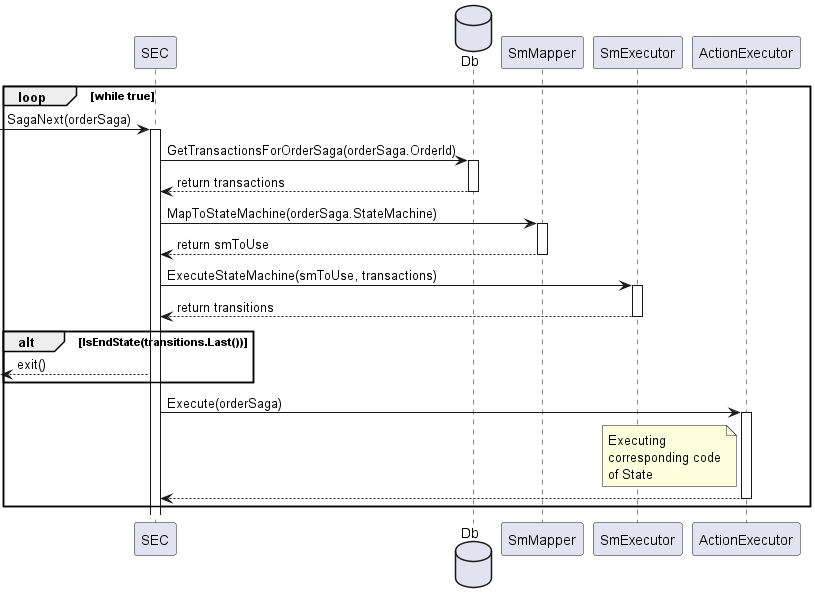
\includegraphics[width=\linewidth]{figures/ChapterVersuchsdurchführung/sec_execution_flow.png}
	\caption{Kontrollfluss der SEC}
	\label{fig:sequence_diagramm_sec_control_flow}
\end{figure}
\FloatBarrier
